	\paragraph{}
	En este capítulo expondremos el trabajo que se pretende realizar para conseguir cada uno de los objetivos mostrados en el capítulo anterior.
	
\section{Objetivo principal del proyecto}

	\paragraph{}
	Se desarrollará una aplicación gráfica multiplataforma, mediante la herramienta \emph{Unity} utilizando el motor gráfico que incluye, para alojar el simulador de tráfico; y se desarrollará una aplicación [TODO: ¿cómo?] para la obtención de mapas de carreteras reales.

\section{Red viaria}

	\paragraph{}
	La red viaria que utilizará el simulador vendrá especificada en un fichero con formato GraphML \cite{GraphML_man}. Dicha red estará determinada por dos grafos, un grafo no dirigido, de topología, en el que los cruces serán los nodos, y las vías serán los arcos; y un grafo dirigido, para indicar los giros, en el que las vías serán los nodos y los giros serán los arcos. Debido a las restricciones que impone la definición de GraphML sobre los identificadores, cada grafo deberá estar en un fichero distinto. Para ello usaremos dos ficheros por cada red viaria, siendo los ficheros *.topology.graphml para el primer tipo de grafo y los ficheros *.turns.graphml para el segundo. El identificador del grafo en cada uno de los ficheros de la pareja de cada grafo será el mismo.
	
	\paragraph{Nodos del grafo de topología}
	
	\paragraph{}
	Debemos distinguir tres tipos:
	\begin{itemize}
		\item \underline{Nodos de cruce}: Representan un cruce de vías típico. El grado de estos nodos es tres o cuatro.
		
		\begin{figure}[H]
			\centering
				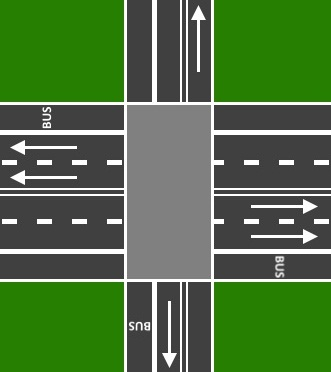
\includegraphics[keepaspectratio,height=100px]{Nodo_cruce.jpg}
		\end{figure}
	
		\item \underline{Nodos de límite de vía}: Representan el límite del área simulada en esa vía y le permitirán al usuario configurar el flujo de tráfico de esa vía (en el caso de que la vía asociada tenga algún carril entrante al área de simulación). El grado de este tipo de nodo es igual a uno.
		
		\begin{figure}[H]
			\centering
				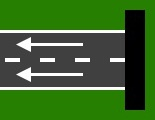
\includegraphics[keepaspectratio,height=50px]{Nodo_limite.jpg}
		\end{figure}
	
		\item \underline{Nodos de continuación}: Representan ángulos en las vías de tal forma que en ellos no se producirán intersecciones de vías. El grado de este tipo de nodo es igual a dos.
		
		\begin{figure}[H]
			\centering
				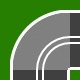
\includegraphics[keepaspectratio,height=50px]{Nodo_continuacion.jpg}
		\end{figure}
	
	\end{itemize}
	
	\paragraph{}
	Por tanto, cada nodo estará definido por un identificador alfanumérico, el tipo de nodo (0: nodo de cruce, 1: nodo de límite de vía, 2: nodo de continuación), sus coordenadas en el plano bidimensional x,y, y para los nodos de tipo cruce, el tipo de cruce, dado que queremos dar la oportunidad al usuario de elegir entre cruce normal (0) o rotonda (1).
	
	\paragraph{Arcos del grafo de topología}	
	\paragraph{}
	Cada arco estará definido por un identificador alfanumérico, el nodo de origen, el nodo de destino, una cadena de texto para poder dar nombre a la vía, y dos cadenas de texto que servirán para indicar los tipos de carril en cada sentido.
	
	\paragraph{}
	Cada una de las cadenas de tipo de carril especificará el tipo de carril o carriles de ese sentido que haya desde el exterior de la vía hacia el interior de la misma utilizando los códigos: P: para indicar un carril de transporte público, N: un carril normal, A: un carril de aparcamiento, V: un carril de Bus/VAO, o la cadena `0' para indicar que no hay carriles en ese sentido.
	
	\paragraph{Nodos del grafo de giros}
	
	\paragraph{}
	Cada nodo estará definido por un identificador alfanumérico que se corresponderá con uno de los identificadores de los arcos del grafo de topología.
	
	\paragraph{Arcos del grafo de giros}
	
	\paragraph{}
	Cada arco estará definido por un identificador alfanumérico, el nodo de origen, el nodo de destino. Si el arco está definido significa que el giro está permitido.
	
	\paragraph{Ejemplo}
	Para ilustrar esta especificación vamos a ver un ejemplo de red viaria y cuál sería su representación en GraphML.
	
	\begin{figure}[H]
		\centering
			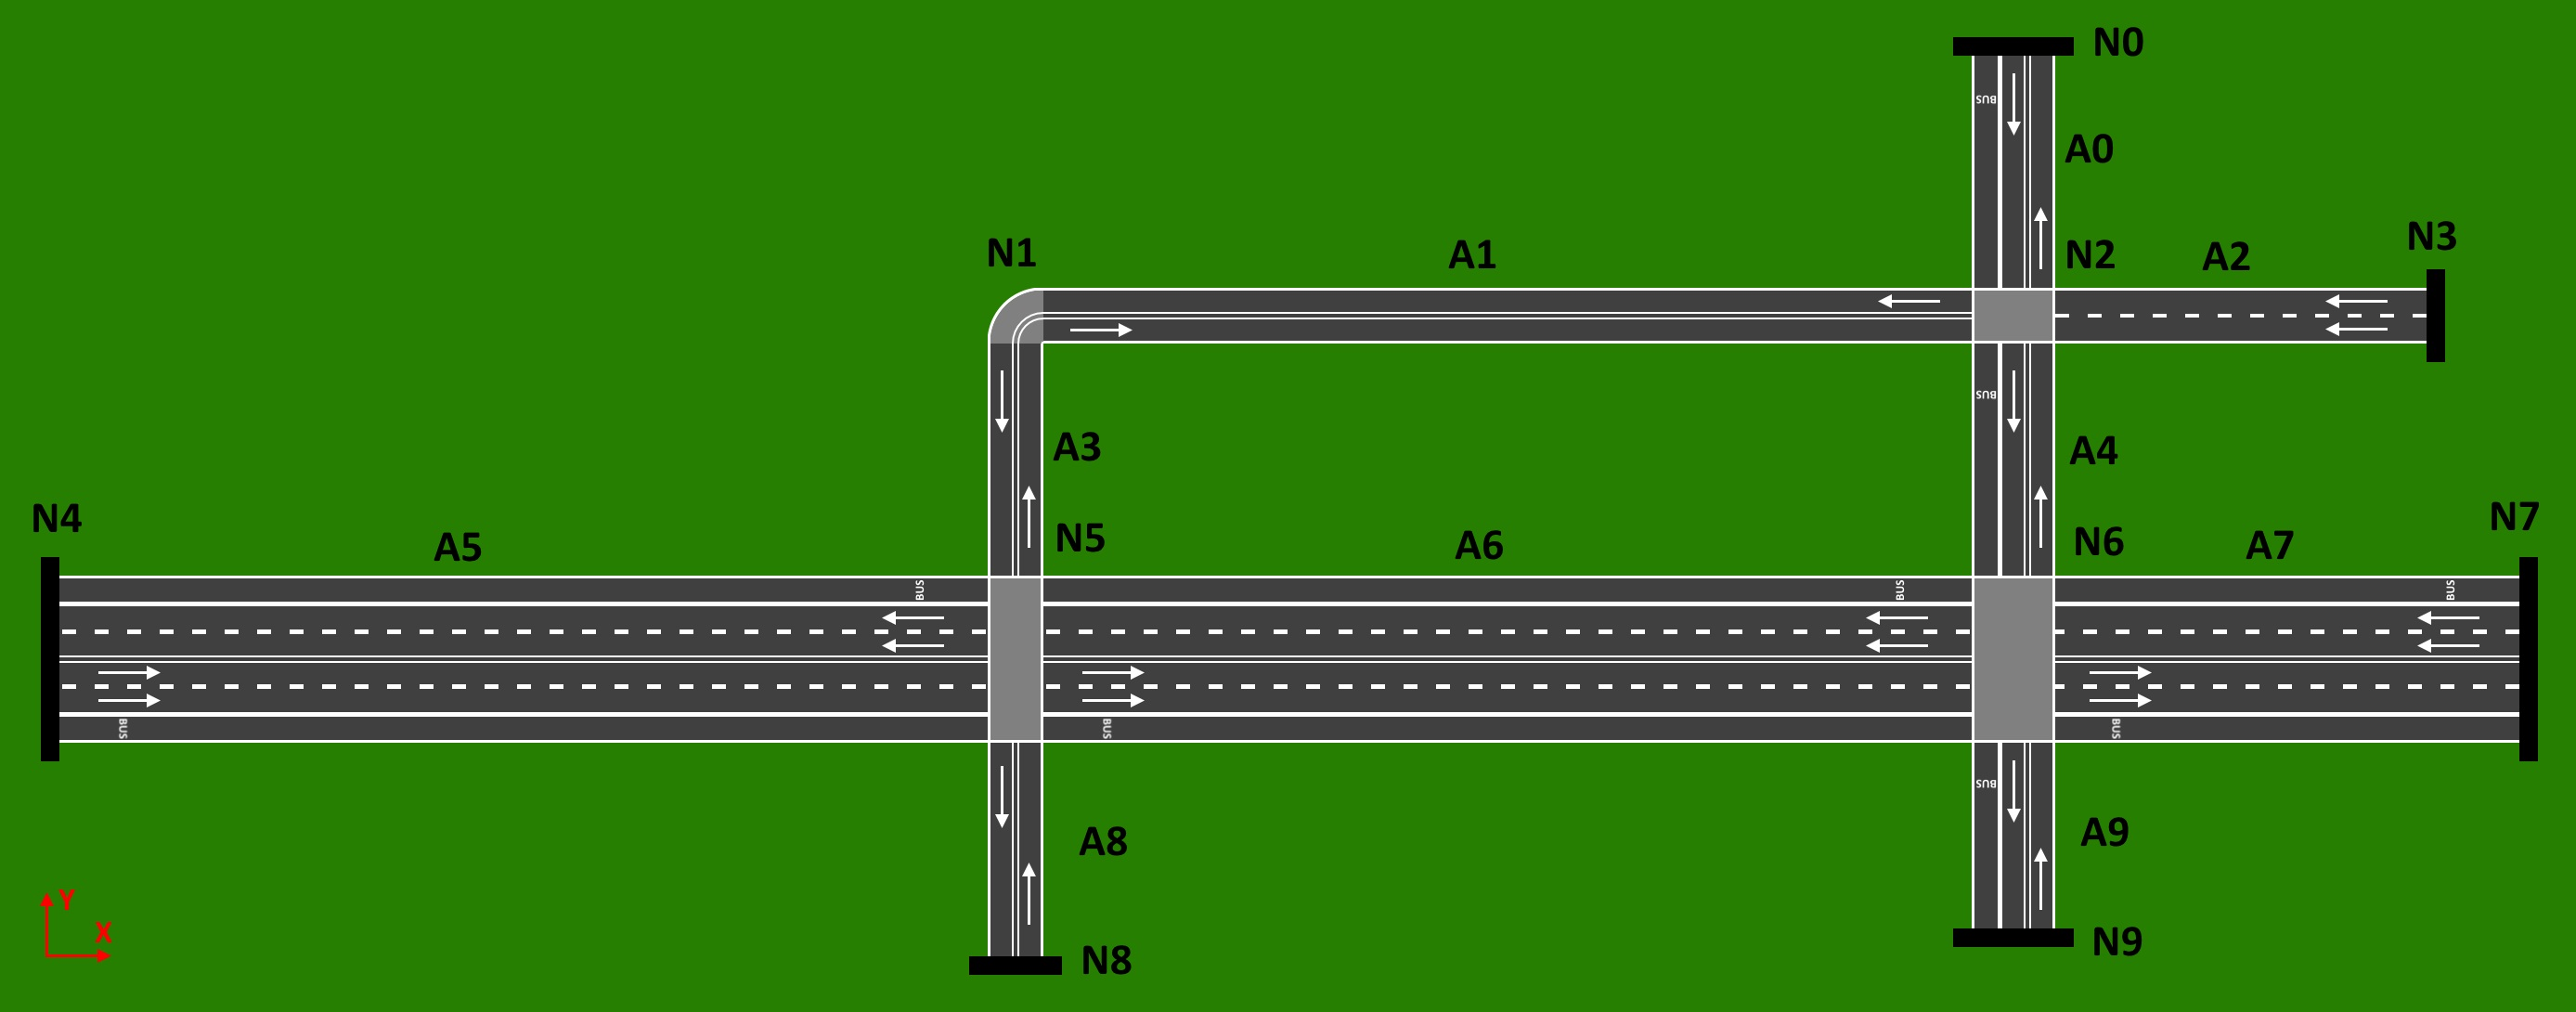
\includegraphics[keepaspectratio,width=359px]{Ejemplo_red_vial.jpg}
	\end{figure}
	
	\paragraph{}
	Como se puede apreciar en la imagen, el grafo de topología asociado consta de diez nodos, tres nodos de tipo cruce, un nodo de tipo continuación y seis nodos de tipo límite de vía. Además, el grafo cuenta con diez arcos que representan las vías de la imagen.
	
	\paragraph{}
	Para este ejemplo se ha supuesto que en cada cruce se puede ir en todas las direcciones que admite esta red, el grafo de giros está compuesto por diez nodos, los arcos del grafo de topología, que en este ejemplo están todos presentes en el grafo debido a que todos están unidos a algún nodo de tipo cruce; y treinta y tres arcos que representan los giros.
	
	\paragraph{}
	A continuación se mostrará la representación de la red viaria con sintaxis de GraphML.
	
	\paragraph{}
	Grafo de topología:
	\tiny
	\lstinputlisting{./code/ejemplo_topologia.graphml}
	\normalsize
	\paragraph{}	
	Grafo de giros:
	\tiny
	\lstinputlisting{./code/ejemplo_giros.graphml}
	\normalsize
	
\section{Señales de tráfico y peatones}

	\paragraph{}
	

\section{Vehículos}
	
	\paragraph{}
	Se importarán los siguientes modelos mediante la herramienta Blender \cite{Blender_web}:
	\begin{itemize}
		\item Bus
		\item Taxi Checker Marathon
		\item Chevrolet Camaro
		\item Todoterreno verde
		\item Todoterreno naranja
		\item Cabeza tractora camión
	\end{itemize}
	
\section{Conductores}

	\paragraph{}
	La lógica de los conductores se realizará mediante una máquina de estados.
	
\section{Entorno}

	\paragraph{}
	
\section{Uso de redes viarias reales}

	\paragraph{}
	